\section{Globales FEM}
Wie in der Aufgabenstellung beschrieben, soll zur Überprüfung der Handrechnungen und zur Bestimmen des Lastpfades ein gloables FEM-Modell zur Anwendung kommen. In diesem Kapitel wird nun beschrieben, wie dieses FEM-Modell aufgesetzt und welche vereinfachende Annahmen getroffen werden. Weiter werden die Ergebnisse der Simulationen aufgeführt und mit den Handrechnungen verglichen und beurteilt.


Analog zu den Handrechnungen werden vier verschiedene FEM-Berechnungen durchgeführt welche jeweils ein Lastfall der Beschleunigung des Modus \emph{A} genauer untersuchen.\\

Mit dem globalen FEM-Modell sollen folgende Punkte bestimmt werden:
\begin{itemize}
  \item Lagerreaktionen
  \item Maximale Axialkräfte, Querkräfte und Biegemomente in Chassis, Dach und den Trägern A und B
  \item Kontaktreaktion: Chassis zu Träger A und B
  \item Kontaktreaktion: Chassis zu Boden
  \item Deformation
\end{itemize}

\subsection{Idealisierung und Modell}
Das FEM-Modell des Solar Butterflys wird, wie in den Handrechnungen, mit Balken und Schlaen idealisiert. Das Chassis, die Deichsel, die Träger A und B sowie die Dachträger werden als Balkenelementen mit den entsprechenden Querschnitten modeliert. Die Wände, Dächer und der Boden werden als Schalenkörper modelliert, wobei den Schalenkörper jeweils ein Lagenaufbau zugewiesen wird, welcher ihre Sandwichbauweise nachstellt. In der Abbildung \ref{FEM Mesh1} ist das komplette Modell des Solar Butterflys dargestellt. In der Abbildung \ref{FEM Mesh3} wurden die Schalenkörper ausgeblendet, sodass nur die Balken sichtbar sind.

\begin{figure}[H]
  \centering
  \centering
  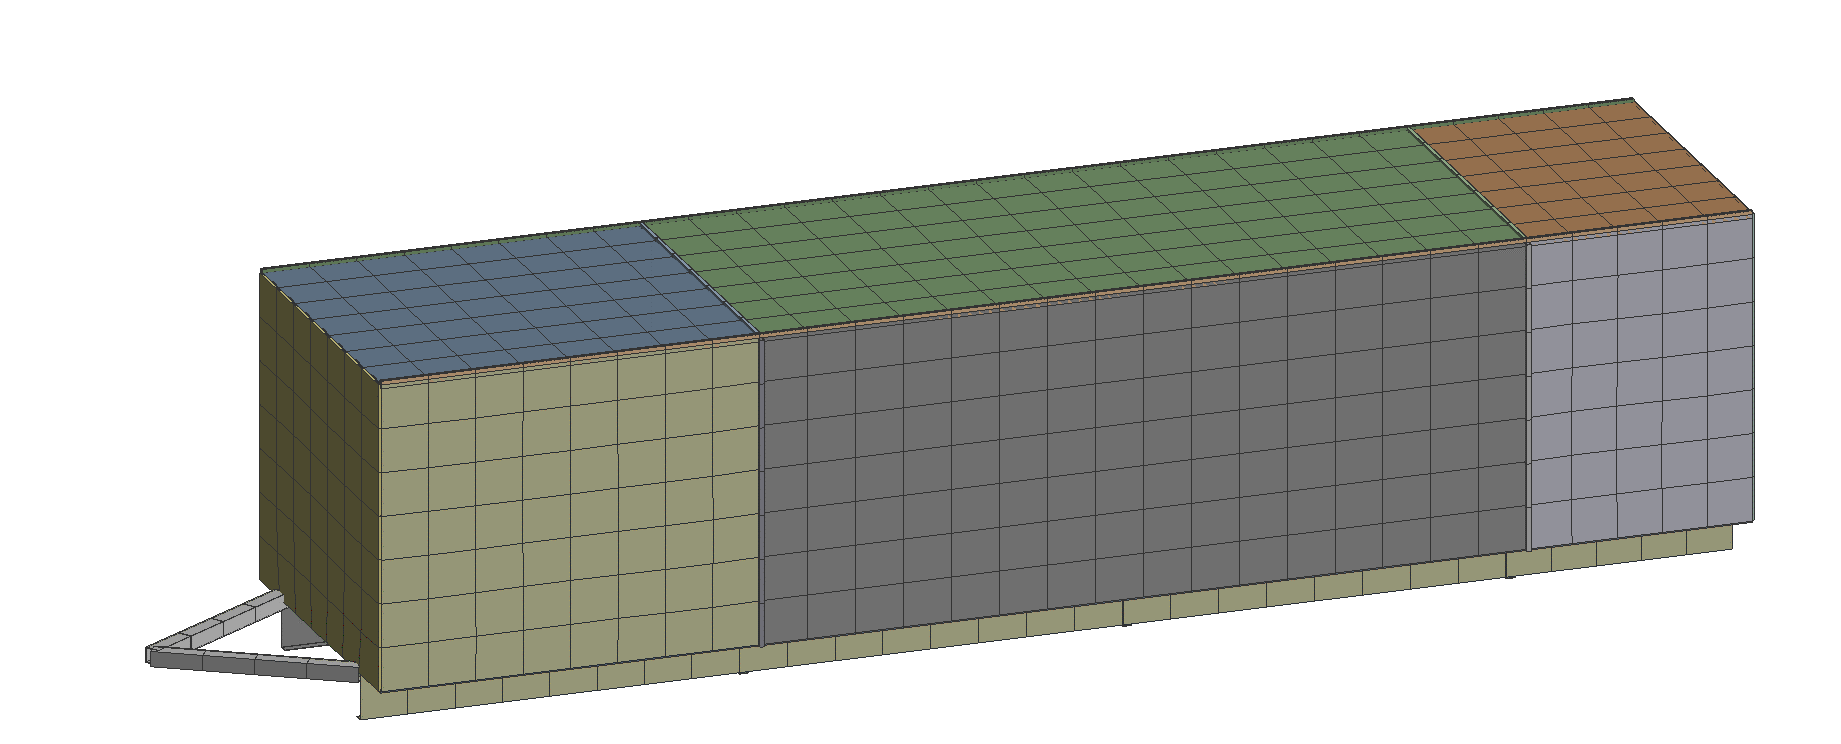
\includegraphics[width=.7\linewidth]{04_figures/FEM Mesh1.png}
  \caption{Darstellung der Balken und Schalenkörper im FEM-Modell}
  \label{FEM Mesh1}
\end{figure}
\begin{figure}[H]
  \centering
  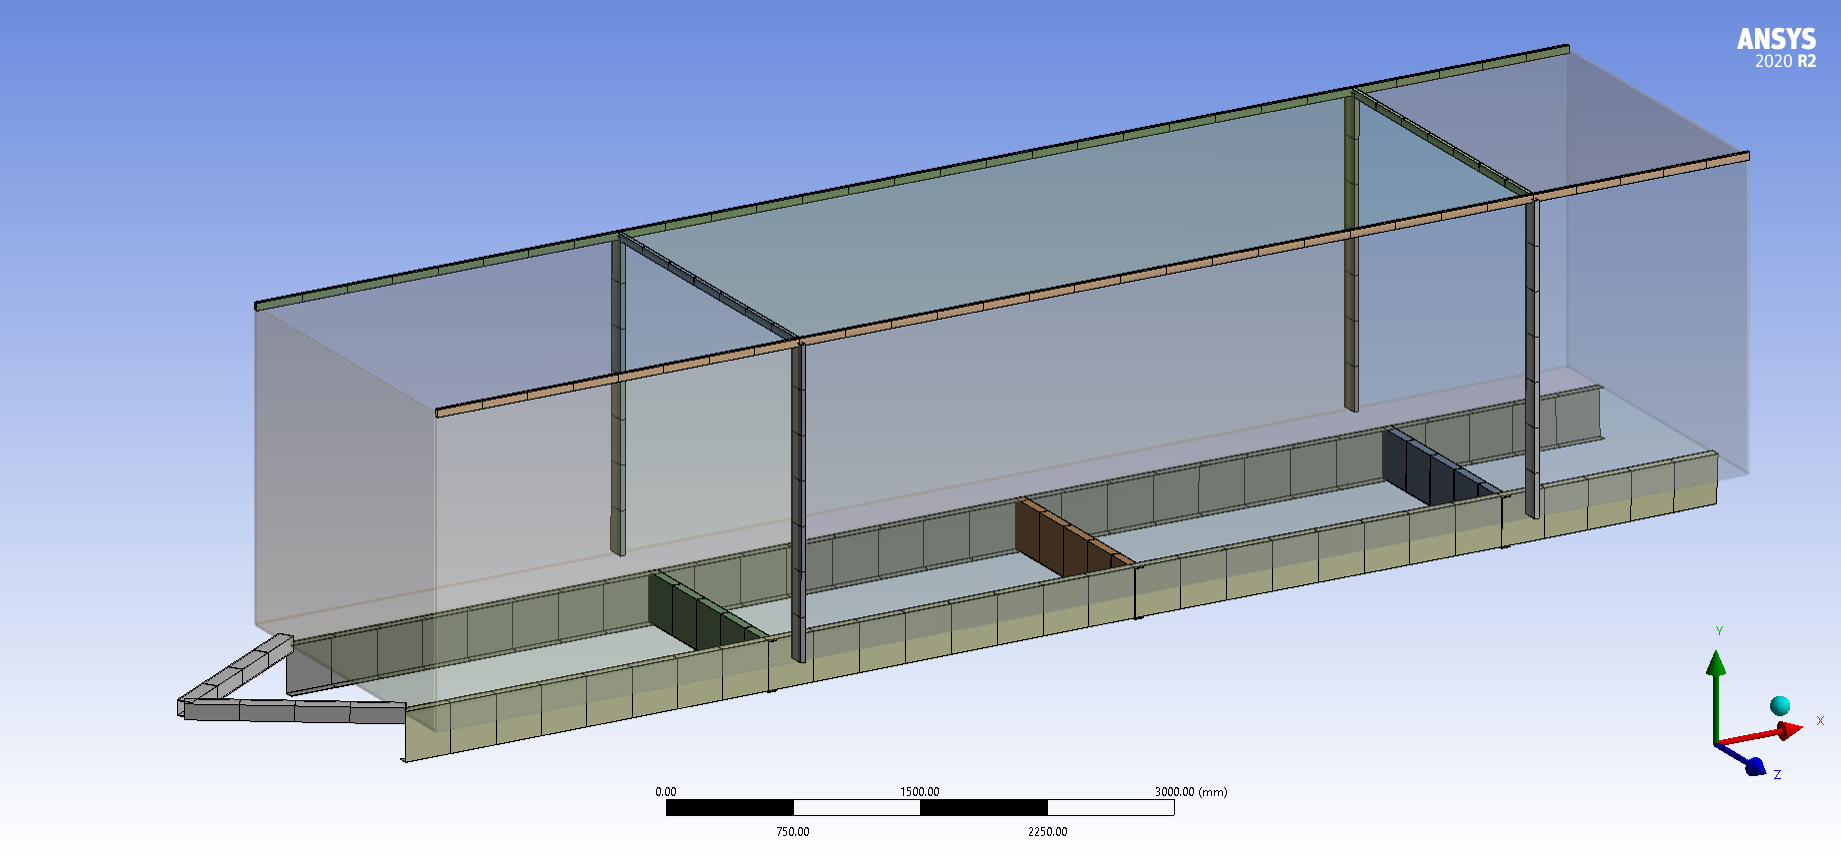
\includegraphics[width=.7\linewidth]{04_figures/FEM Mesh3.png}
  \caption{Darstellung der als Balken idealisierten Körper}
  \label{FEM Mesh3}
\end{figure}

Um die Masse des Solar Butterflys modellieren zu können, werden, zusätzlich zu den Massen der modellierten Bauteilen, Punktmassen (Point-mass) eingeführt. Es werden für die drei Raumelemente Küche, Mittelkörper und Bad je eine Punktmasse definiert, deren Masse und Trägheitsmomente mit der Hilfe der Massenverteilung aus dem Kapitel \ref{Massenverteilung} bestimmt werden. In der Abbildung \ref{img:FEM Punktmasse} sind die Verbindungen der Punktmassen mit dem Rest des Modelles dargestellt. Sie werden über das Chassis, die Träger A und B, sowie über die Verbindungsstellen wischen den Wänden und dem Boden getragen.\\
\begin{figure}[H]
  \centering
  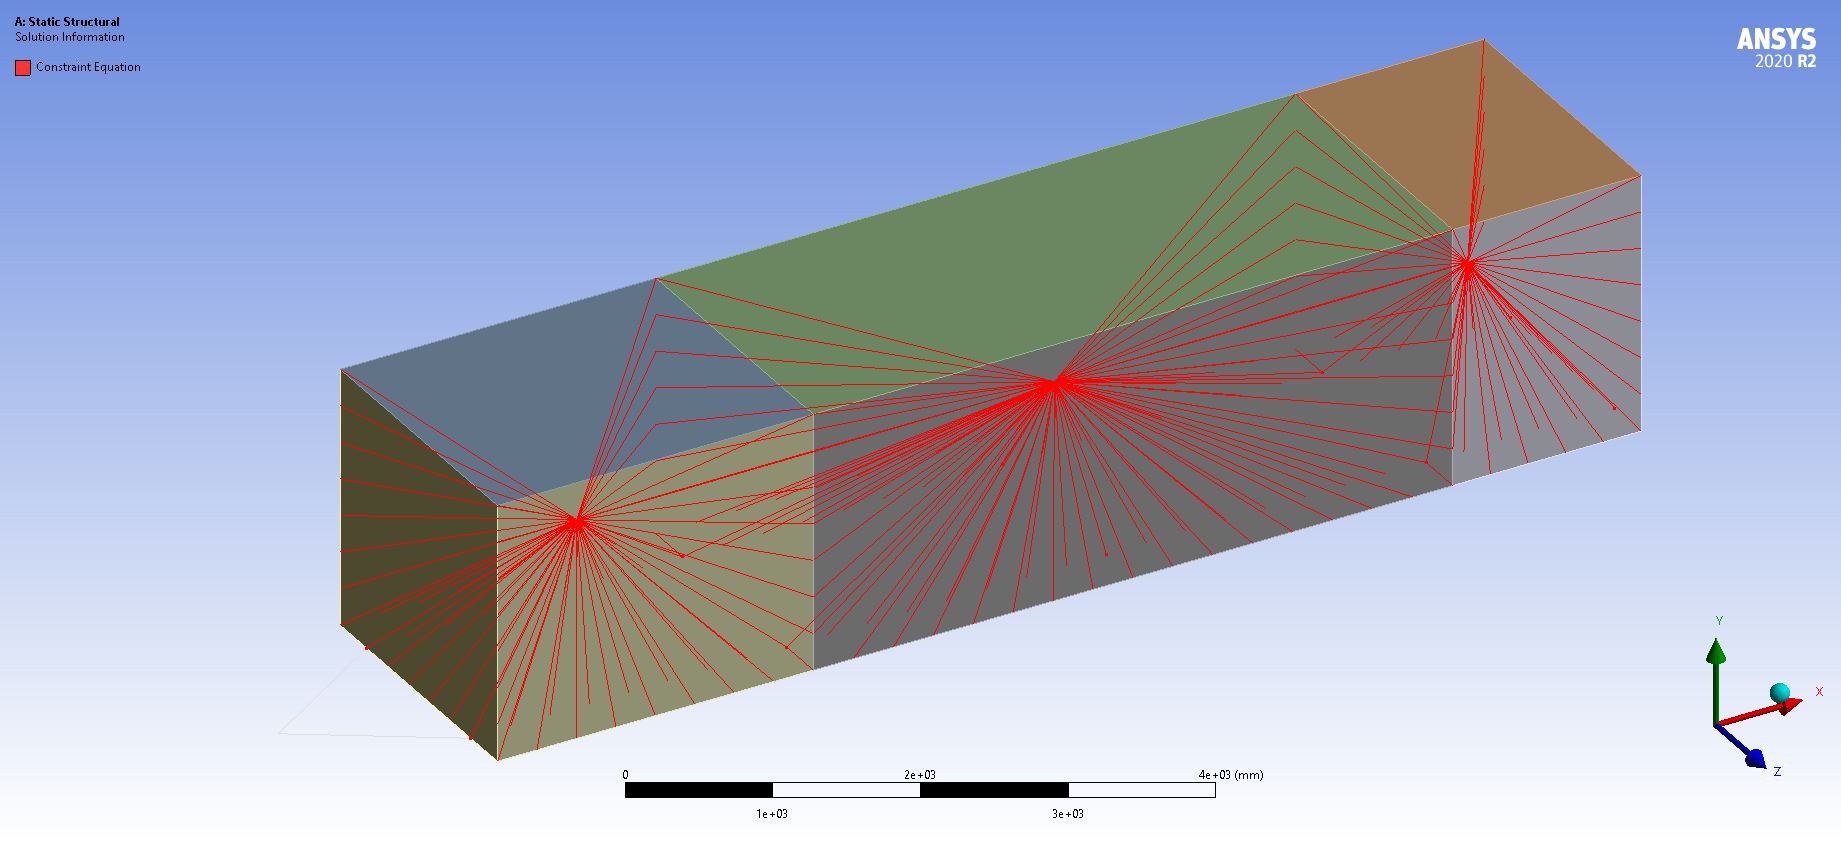
\includegraphics[width=0.7\linewidth]{04_Figures/FEM Punktmasse.png}
  \caption{Verbindungen der Punktmassen zum Rest des Modelles}
  \label{img:FEM Punktmasse}
\end{figure}

Die Deichsel, Längsträger und Querträger des Chassis werden durch das Zusammenführen der deckungsgleichen Koten miteinander verbunden. Auf die selbe Art und Weise werden die Träger A und B, die Träger des Daches sowie der Boden, die Wände und das Dach des Aufbaus miteinander verbunden. Der verbundene Aufbau wiederum wird auf zwei Arten mit dem Chassis verbunden. Einerseits werden die Träger A und B über einen \emph{Fix-Joint} (alle Freiheitsgrade eingeschränkt) an ihrem untersten Knoten mit dem Chassis verbunden. Weiter wird der Boden über \emph{General-Joint}-Verbindungen
\footnote{Die General-Joints wurden mit der Hilfe einer \emph{Named Selection} und dem \emph{Object-Generation} Menu erstellt. Die Kraftreaktionen wurden durch die Parametrisierung der Ergebnisse ausgelesen.}
(die rotatorischen Freiheitsgrade sind frei, die translatorischen eingeschränkt.) mit den Längsträgern des Chassis verbunden. Insgesammt ist der Boden an jedem Längsträger über 30 Knotenverbindungen it dem Chassis verbunden. Sie räpresentieren die Klebestellen zwischen Boden und Chassis. Mit dem Auslesen der Kontaktreaktionen dieser beiden Verbindungen können Aussagen bezüglich der Verbindung zwischen den Trägern A und B und dem Chassis, sowie auch der Klebestelle zwischen dem Chassis und Boden gemacht werden.\\
In allen folgenden beschriebenen FEM-Simulationen ist der Solar Butterfly analog zu den Handrechnungen im Kapitel \ref{sub:Longitudinale Beschleunigung} (Lastfall \emph{1.1 Vertikale Beschleunigung}) gelagert. Am Spitz der Deichsel sind die rotatorischen Freiheitsgrade frei, die translatorischen jedoch eingeschränkt. An der Achse wird lediglich die Verschiebung in x-Richtung (Fahrtrichtung) zugelassen.

\subsection{Ergebnisse}
Im Anhang \ref{FEM Ergebnisse} sind die Ergebnisse der FEM-Berechnungen Tabelarisch festgehalten. Sofern für die ausgelesenen Grössen Handrechnungen durchgeführt wurden, sind deren Ergebnisse ebenfalls in den besagten Tabellen zu finden, sodass diese direkt mit den Ergebnissen der FEM-Berechnungen verglichen werden können. Die Schnittkräfte und Kontaktreaktionen der Tabellen beziehen sich jeweils auf einen einzelnen Balken oder Verbindungsstelle. Die Kontaktreaktion zwischen Chassis und Boden bezieht sich auf eine einzelne Knotenverbindung. Die in den Tabellen aufgeführten Werte stellen jeweils den Maximalwert dar.\\
Im Anhang \ref{FEM Deformation} sind Bilder, welche die Deformation des Solar Butterflys dokumentieren, zu finden. Die FEM-Datei ist im elektronischen Anhang ANHANG angefügt. Die Auswertung der Ergebnisse wurde mit einer Exceltabelle durchgeführt, welche im elektronsichen Anhang AHNAHNG zu finden ist.


\subsubsection{Vergleich mit Handrechnungen}
Im Lastfall \emph{1.1 Vertikale Beschleunigung} sind die berechneten Axialkräfte (xx kN) im Dach rund doppelt so hoch, wie jene des FEM-Modelles (xx kN). Dies ist vermutlich darauf zurück zu führen, dass das mittragende Dach, welches ebenfalls Axialkräfte aufnimmt, in den Handrechnungen nicht mit berücksichtigt wurde.\\
Im Lastfall \emph{1.4 Laterale Beschleunigung} sind die mit der FEM-Berechnung erhaltenen Axialkräfte im Chassis und den Längsträger des Daches gut drei mal höher als jene der Handrechnungen. Dies, da sich der Solar Butterfly unter lateraler Beschleunigung, nicht wie angenommen verbiegt, sondern verdreht. Die Art der Deformation ist ähnlich wie jene im Lastfall \emph{1.5 Rotatorische Beschleunigung} (vgl. Abbildungen \ref{FEM 1.4} und \ref{FEM 1.5} im Anhang \ref{FEM Deformation}). Da diese grundlegende Annahme der Auswirkungen der Belastung (und der Deformation) falsch getroffen wurde, sind die Ergebnisse auch dem entsprechend unterschiedlich. Die erhaltenen Kräfte sind in ihrer Art vergleichbar mit jenen des Lastfalles \emph{1.5 Rotatorische Beschleunigung}, im Betrag liegen sie jedoch tiefer.\\
Abschliessend kann zum Vergleich gesagt werden, dass die FEM-Ergebnisse plausieble sind.

\subsubsection{Beurteilung Dach}
In der folgenden Tabelle sind die Schnittgrössen der Träger des Daches enthalten.

\begin{table}[H]
\centering
\begin{tabular}{lccccccc}
\thickhline
&	Einheit	&	1.1	&	1.3	&	1.4	&	1.5	&	Max	&	Min	\\	\hline
Axialkraft	&	N	&	2879	&	-1562	&	-2560	&	-3625	&	2879	&	-3625	\\
Querkraft	&	N	&	108	&	56	&	24	&	32	&	108	&	24	\\
Biegemoment	&	kNmm	&	42	&	17	&	13	&	19	&	42	&	13	\\	\thickhline
\end{tabular}
\caption{Schnittgrössen in den Trägern des Daches in den unterschiedlichen Lastfällen}
\label{tab:FEMres Dach}
\end{table}

Wie im Kapitel \ref{Dach} beschrieben, ist das dimensionierende Kriterium des Daches dessen Verformung aufgrund des Eigengewichtes. Dem entsprechend stellen die in der Tabelle \ref{tab:FEMres Dach} aufgeführten Schnittgrössen keine kritischen Lasten dar.

Das Potential der Gewichtsoptimierung wird als gering eingestuft. Auch wenn die Träger des Daches global gesehen überdimensioniert sind, werden über sie, im eingefahrenen Zustand, die ausfahrbaren Seitenmodule befestigt und gesichert. Würde ein anderes Konzept zur Versperrung der ausfahrbaren Seitenmodulen ausgearbeitet, könnte das Dach eventuell auf eine andere Weise versteift (z.B. mit aufgeklebten CFK-Hutprofilen) und die Dachträger weggelassen werden.\\
Wird vom jetzigen Konzept noch weiter abgewichen und das Konzept des unterbrochenen Daches (4 GFK-Sandiwichpanelen à ca. 2 x 1.3 m im Mittelkörper) verworfen, gäbe es allenfalls die Möglichkeit, ein durchgehendes Dach in Sandwichbauweise zu verwenden. Dieses könnte, ähnlich wie der Boden, mit Ocean-PET und Aluminium Deckschichten in einem Stück gefertigt und mit Hartschaum-Einsätzen und Verstärkungen individuell angepasst und optimiert werden. Der Nachteil diese Konzeptes ist jedoch, dass nicht die Standard-Solarmodule verwendet werden können, welche von Begin an des Projektes als vorgegeben betrachtet wurden (Sponsoring). Es stellt sich entsprechend die Frage, zum einen \emph{wer} und \emph{wie} die Solarzellen auf das Dach laminiert werden, da diese nicht direkt im Herstellungsprozess der Sandwichkonstuktion mitlaminiert werden können. Dass die Solarzellen unter Umständen ``von Hand'' auf das Dach laminiert werden müssen, könnte sich aufgrund der Flexibilität bezüglich Dimensionen und Verkabelung, auch als Vorteil erweisen. Als weiterer Vorteil ist zu ergänzen, dass die Verbindungsstellen zwischen den Solarpanelen und Träger, sowie zwischen den einzelnen Solarpanelen, wegfallen würden.\\
Auch wenn die Gewichtsersparnisse vermutlich gering sind (oder wohl möglich auch nicht vorhanden sind), würde die Komplexität des Daches potenziell reduziert werden können.



\subsubsection{Beurteilung Träger A und B}
In der Tabelle \ref{tab:FEMres Träger} sind die maximalen Schnittgrössen der Träger A und B zusammengestellt.
\begin{table}[H]
\centering
\begin{tabular}{lccccccc}
\thickhline
&	Einheit	&	1.1	&	1.2	&	1.4	&	1.5	&	Max	&	Min	\\	\hline
Axialkraft	&	N	&	-10904	&	-1562	&	2684	&	-4119	&	2684	&	-10904	\\
Querkraft	&	N	&	1293	&	56	&	1067	&	1311	&	1311	&	56	\\
Biegemoment	&	kNmm	&	327	&	17	&	627	&	772	&	772	&	17	\\	\thickhline
\end{tabular}
\caption{Schnittgrössen der Träger in den unterschiedlichen Lastfällen}
\label{tab:FEMres Träger}
\end{table}

Die maximale Axialkraft von -10.9 kN hat, bei einer Querschnittsfläche eines Trägers von rund 1180 $mm^2$, Druckspannungen von 9.2 MPa zur folge. Die Gefahr des Knickens ist nicht vorhanden, da die Träger auf mindestens zwei Seiten über die Wände gestützt werden und die Druckbelastung im verhältniss zum Flächenträgheitsmoment des Trägers eher tief ist (Knickung nach Euler). Das Maximale Biegemoment von 772 kNmm führt, bei einem minimalen Widerstandsmoment von 11900 $mm^3$, zu Spannungen in der höhe von 65 MPa.\\
Ob die Dimensionen der Träger A und B optimal gewählt wurden lässt sich anhand der FEM-Ergebnissen nicht beurteilen, da angenommen wird, dass die dimensionierenden Belastungen währen dem Ausfahren der Seitenmoudlen (Modus B3) auftreten. Wie im Kapitel KAPITEL vorgeschlagen, wird unter anderem empfohlen in einem weiteren Schritt ein globales FEM-Modell für den Modus B3 zu erstellen und dieses zu analysieren. Es kann jedoch gesagt werden, dass die überprüften Lastfälle keine kritischen Belastungen für die Träger A und B darstellen, diese jedoch auch nicht überdimensioniert sind. Dem entsprechend kann das Potential zur Gewichtseinsparung nur bedingt abgeschätzt werden.

\subsubsection{Verbindung Boden zu Chassis}
In der folgenden Tabelle sind die maximalen Kontaktreaktion der Verbindung zwischen Chassis und Boden zu finden. Die Ergebnisse beziehen sich jeweils auf eine der insegsammt 60 Knotenverbindung.

\begin{table}[H]
\centering
\begin{tabular}{lcccccc}
\thickhline
&	Einheit	&	1.1	&	1.2	&	1.4	&	1.5	&	Max	\\	\hline
Normalkraft (Zug)	&	N	&	883	&	35	&	1942	&	3118	&	3118	\\
Schubkraft (xz-Ebene)	&	N	&	9933	&	1733	&	10972	&	10761	&	10972	\\	\hline
Normalspannungen	&	MPa	&	0.06	&	0.00	&	0.13	&	0.21	&	0.21	\\
Schubspannungen	&	MPa	&	0.67	&	0.12	&	0.74	&	0.72	&	0.74	\\	\thickhline
\end{tabular}
\caption{Schnittgrössen und Spannungen der Verbindung zwischen Chassis und Boden in den unterschiedlichen Lastfällen}
\label{tab:FEMres Boden}
\end{table}

Wird die Klebefläche des Chassis auf die 60 Knotenverbindungen verteilt ergibt sich eine Fläche von 999999 $mm^2$ pro Verbindung. Mit den in der Tabelle \ref{tab:FEMres Boden} angegebenen Kontaktreaktionen ergeben sich maximale Normalspannungen von x.xx MPa und maximale Schubspannungen von x.xx MPa, welche beide unterhalb der Design-Allowables liegen. 

Bei einer Fläche von 17880 $mm^2$ pro Abschnitt ergibt sich eine maximale Normalspannung von 0.04 MPa und eine maximale Schubspannung von 0.54 MPa. Beide Werte liegen deutlich unterhalb des Design-Allowable. Hierbei muss jedoch angemerkt werden, dass lokal die Spannungen deutlich höher liegen könnten und, dass das verwendete Modell nicht geeignet ist um diese Spannungskonzentrationen zu erkennen.

\subsubsection{Verbindung Träger A und B zu Chassis}
\begin{table}[H]
\centering
\begin{tabular}{lccccc}
\thickhline
Lastfall / Träger	&	Einheit	&	x	&	y	&	z	&	total	\\	\hline
1.1 A	&	\multirow{8}{*}{N}	&	-56	&	2084	&	325	&	2110	\\
1.1 B	&		&	98	&	667	&	80	&	679	\\
1.2 A	&		&	-56	&	2084	&	325	&	2110	\\
1.2 B	&		&	98	&	667	&	80	&	679	\\
1.4 A	&		&	237	&	-3577	&	1729	&	3979	\\
1.4 B	&		&	-733	&	-4221	&	1679	&	4602	\\
1.5 A	&		&	373	&	-5525	&	2346	&	6014	\\
1.5 B	&		&	-1309	&	-6399	&	2221	&	6899	\\	\hline
Max	&		&	373	&	2084	&	2346	&	6899	\\
Min	&		&	-1309	&	-6399	&	80	&	679	\\	\thickhline
\end{tabular}
\caption{Maximale Axialkräfte in den Trägern A und B in den unterschiedlichen Lastfällen}
\label{tab:FEMres Träger Axial}
\end{table}

\begin{table}[H]
\centering
\begin{tabular}{lccccc}
\thickhline
Lastfall / Träger	&	Einheit	&	x	&	y	&	z	&	total	\\	\hline
1.1 A	&	\multirow{8}{*}{kNmm}	&	-734	&	-19	&	2	&	734	\\
1.1 B	&		&	-236	&	34	&	-14	&	238	\\
1.2 A	&		&	-734	&	-19	&	2	&	734	\\
1.2 B	&		&	-236	&	34	&	-14	&	238	\\
1.4 A	&		&	1924	&	71	&	-102	&	1928	\\
1.4 B	&		&	2097	&	-251	&	95	&	2114	\\
1.5 A	&		&	2767	&	112	&	-164	&	2774	\\
1.5 B	&		0	2996	&	-452	&	159	&	3034	\\	\hline
Max	&		&	2996	&	112	&	159	&	3034	\\
Min	&		&	-734	&	-452	&	-164	&	238	\\	\thickhline
\end{tabular}
\caption{Maximale Biegemomente in den Trägern A und B in den unterschiedlichen Lastfällen}
\label{tab:FEMres Träger Moment}
\end{table}


\subsubsection{Deformationen}
Die FEM-Berechnungen zeigen, dass das Chassis, im Bezug auf das Übernehmen von Lasten, eine wichtigere Funktion übernimmt, als zuvor angenommen. Die Funktion es Aufbaus wurde wiederrum überschätzt. Diese Feststellung lässt sich unteranderem an den Abbildungen \ref{} und \ref{} anhand den Deformationen erkennen. Das Chassis verformt sich realtiv stark, während der Aufbau seine rechteckige Form nahezu bei behält. Besonders in den Lastfällen der lateralen und rotatorischen Beschleunigung ist zu erkennen, dass sich lediglich das Chassis stark verdreht, und nicht wie angenommen der komplette Körper. Dies zeigt, dass die Eigenschaft des Chassis bezüglich Steifigkeit, im Vergleich zum Aufbau, eine entscheidende Rolle spielt. \\

Es ist jedoch nicht klar, ob dieses Ergebniss zum Teil auch auf die Art der Einbindung der Punktmassen zurück zu führen ist. Oder anderst ausgedrückt: es ist nicht klar, ob das selbe Ergebnis erzielt werden könnte, wenn die Massen realitätsgetreuer modelliert und ins Modell eingebunden worden wären. So befindet sich in der Realität ein grösserer Teil der Masse, in Form der ausfahrbaren Solarmodulen und den dazugehörigen Antriebselementen, an den Wänden des Solar Butterflys und nicht, wie modelliert, in den Zentern der Raumelemente.
Die Masse der ausfahrbaren Solarmodulen muss über die Wände und Träger A und B, zu einem gewissen Ausmass auch über das Dach, getragen und dessen Trägheitskräfte auf das Chassis übertragen werden. Die Punktmassen sind jedoch fast ausschliesslich direkt über das Chassis und die Träger A und B befestigt worden. Durch eine exaktere Verteilung und Einbindung der Massen ins Modell, würde sich der Lastpfad entsprechend verändern, was andere FEM-Ergebnisse hervor bringen würde.
Es ist wahrscheinlich, dass der Aufbau in der realität eine tragendere Funktion übernimmt, als dies durch die FEM-Berechnungen gezeigt wird und dass dessen Deformation stärker ausfallen würde.\\
Auch wenn mit einer exakteren Modellierung gezeigt werden könnte, dass der Aufbau eine wichtigere Rolle übernimmt als dies durch die vorliegenden FEM-Berechnungen nahe gelegt wird, steht fest, dass die Eigenschaften des Chassis das Verhalten des Solar Butterflys dominieren.\\

Das Gewicht des Chassis beansprucht mit 650 kg ??? rund ein Viertel der Gewichtslimite für Europa von 2200 kg. Weiter handelt es sich beim Chassis um ein ``Standard-Chassis'', welches nicht spezifisch für die Anwendung in diesem Projekt ausgelegt und optimiert wurde. Ferner wird der Boden zur Zeit nicht optimal ausgenützt. So entspringt die dimensionierende Grösse des Bodens aus einem Missbrauchslastfall (``Spitzer Schuh'') und nicht aus dessen Funktion als tragendes Strukturelement. In der Ausarbeitung des Konzeptes wurde der Boden als einzelnes Bauteil, und nicht, in Verbindung mit dem Chassis, als integraler Bestandteil der tragenden Struktur betrachtet. Folglich wird das grösste Potential zur Gewichtsreduktion im Bereich der Grundstruktur, in der Optimierung des Chassis in Kombination mit dem Boden gesehen.\\
Es ist zu vermuten, dass durch die Optimierung die Klebeverbindung zwischen Chassis und Boden noch stärker beansprucht werden würde, als dies bereits der Fall ist. Ob eine Klebeverbindung noch immer eine angemessene Wahl ist, müsste in der Optimierung genauer beurteilt werden.
\newpage
